\documentclass[aspectratio=169,11pt,t]{beamer}
% ============================================================
%  ksa-cs-v2: ksa-cs-lecture-template.tex 스타일 + 한글, v2 덱(16:9)용.
%    - 짙은 네이비 헤드라인 (섹션 이름 + 프레임마다 점)
%    - 꽉 찬 파란 제목 막대, 둥근 그림자 블록
%    - 한글: Noto Sans CJK KR (fontspec)
%  사용:
%    \documentclass[aspectratio=169,11pt,t]{beamer}
%    \input{<..>/theme/ksa-cs-v2.tex}
%  ksa-theme.tex 의 매크로(\kb \kq, ksablue/ksared 등)도 같은 이름으로 둔다
%  -> v2 덱 본문을 거의 그대로 옮길 수 있다.
% ============================================================

\usepackage{fontspec}
\usepackage{amsmath,amssymb}
\usepackage{tikz}
\usepackage{listings}
\usepackage{graphicx}
\usepackage{booktabs}
\usepackage{varwidth}
% enumitem 은 넣지 않는다 (beamer 글머리표가 사라진다)

\defaultfontfeatures{Ligatures=TeX}
\setmainfont{Noto Sans CJK KR}
\setsansfont{Noto Sans CJK KR}
\setmonofont{Noto Sans Mono CJK KR}[Scale=0.92]
\usefonttheme{professionalfonts}

% ---------- 기본 틀 ----------
\usetheme{default}
\useinnertheme[shadow=true]{rounded}
\setbeamertemplate{navigation symbols}{}
\setbeamersize{text margin left=1em,text margin right=1em}

% ---------- 색 (템플릿 원본 값) ----------
\definecolor{navydark}{HTML}{191959}
\definecolor{navydim}{HTML}{8888B0}
\definecolor{navytitle}{HTML}{262686}
\definecolor{navyblue}{HTML}{3333B2}
\definecolor{blockbodybg}{HTML}{E9E9F3}
\definecolor{examplegreen}{HTML}{006000}
\definecolor{examplebg}{HTML}{E5EFE5}
\definecolor{alertred}{HTML}{BF0000}
\definecolor{alertbg}{HTML}{F9E5E5}
% ksa-theme.tex 와 같은 이름 (본문 호환)
\colorlet{ksablue}{navytitle}
\colorlet{ksabluedk}{navydark}
\definecolor{ksagold}{HTML}{D6CBB1}
\definecolor{ksagolddk}{HTML}{A9976B}
\colorlet{ksared}{alertred}
\definecolor{ksagray}{HTML}{5B5B5B}

\setbeamercolor{structure}{fg=navyblue}
\setbeamercolor{alerted text}{fg=alertred}
\setbeamercolor{frametitle}{bg=navytitle,fg=white}
\setbeamercolor{title}{fg=white,bg=navytitle}
\setbeamercolor{block title}{bg=navytitle,fg=white}
\setbeamercolor{block body}{bg=blockbodybg,fg=black}
\setbeamercolor{block title example}{bg=examplegreen,fg=white}
\setbeamercolor{block body example}{bg=examplebg,fg=black}
\setbeamercolor{block title alerted}{bg=alertred,fg=white}
\setbeamercolor{block body alerted}{bg=alertbg,fg=black}
\setbeamercolor{item}{fg=navyblue}
\setbeamertemplate{itemize item}[circle]
\setbeamertemplate{itemize subitem}[triangle]

% ---------- 헤드라인: miniframes (섹션 이름 + 점) ----------
\useoutertheme[subsection=false]{miniframes}
\setbeamerfont{section in head/foot}{size=\tiny}
\setbeamercolor{section in head/foot}{bg=navydark,fg=white}
\setbeamercolor{mini frame}{fg=white}
\setbeamertemplate{mini frames}[circle]

% ---------- 제목 막대: 폭 꽉 채움, 두 줄까지 ----------
\setbeamerfont{frametitle}{size=\normalsize,series=\bfseries}
\setbeamertemplate{frametitle}{%
  \nointerlineskip
  \begin{beamercolorbox}[wd=\paperwidth,ht=2.7ex,dp=1.1ex,leftskip=.3cm,rightskip=.3cm]{frametitle}%
    \usebeamerfont{frametitle}\insertframetitle
  \end{beamercolorbox}}

% ---------- 쪽 번호: 오른쪽 아래 ----------
\setbeamertemplate{footline}{%
  \hfill
  {\color{navydim}\scriptsize\insertframenumber\,/\,\inserttotalframenumber}%
  \hspace{3mm}\vspace{2mm}%
}

% ---------- 표지: 템플릿처럼 헤드라인은 그대로, 가운데 둥근 그림자 상자에 제목 한 줄 ----------
% 덱에서:  {\setbeamertemplate{footline}{}\begin{frame}[c,noframenumbering]\titlepage\end{frame}}
\setbeamercolor{title}{fg=white,bg=navyblue}
\makeatletter
\setbeamertemplate{title page}{%
  \vfill
  \centering
  \begin{minipage}{0.84\paperwidth}
  \begin{beamercolorbox}[wd=\linewidth,sep=7pt,center,rounded=true,shadow=true]{title}
    {\usebeamerfont{title}\inserttitle\par}%
    \ifx\insertsubtitle\@empty\else\vskip0.4em{\usebeamerfont{subtitle}\insertsubtitle\par}\fi
  \end{beamercolorbox}
  \end{minipage}\par\vskip1.6em
  {\usebeamerfont{author}\color{navytitle}\insertauthor\par}\vskip0.3em
  {\usebeamerfont{institute}\color{ksagray}\insertinstitute\par}
  \vfill
}
\makeatother
\setbeamerfont{title}{series=\bfseries,size=\Large}
\setbeamerfont{subtitle}{size=\normalsize}
\setbeamerfont{author}{size=\normalsize}
\setbeamerfont{institute}{size=\small}

% ksa-theme 호환: 덱이 \renewcommand{\ksacredit}{..} 를 해도 되게 (꼬리말에는 안 쓴다)
\newcommand{\ksacredit}{}

% ---------- 강조 ----------
\newcommand{\hl}[1]{\textcolor{alertred}{#1}}
\newcommand{\hlb}[1]{\textcolor{navyblue}{#1}}
\newcommand{\kb}[1]{\textbf{\color{ksablue}#1}}
\newcommand{\kq}[1]{\textbf{\color{ksared}#1}}

% ---------- 파이썬 코드 (템플릿과 같은 색) ----------
\definecolor{codekw}{HTML}{0033B3}
\definecolor{codebuiltin}{HTML}{BF0000}
\definecolor{codestr}{HTML}{067D17}
\definecolor{codecomment}{HTML}{8C8C8C}
\definecolor{codenum}{HTML}{1750EB}
\lstdefinestyle{py}{
  language=Python, basicstyle=\ttfamily\scriptsize,
  keywordstyle=\color{codekw}\bfseries, stringstyle=\color{codestr},
  commentstyle=\color{codecomment}\itshape, numberstyle=\color{codenum},
  emph={print,len,range,sum,input,int,str,float,list,dict,append,remove,sorted,abs,min,max},
  emphstyle=\color{codebuiltin}, showstringspaces=false, keepspaces=true,
  columns=fixed, basewidth=0.52em, aboveskip=1mm, belowskip=1mm, xleftmargin=2mm,
  breaklines=true
}
\lstset{style=py}

% 원본 덱 (ksa-theme): slides/v2/ml1/week09/dropout/ -- 그림은 거기 figs/ 를 그대로 쓴다
\setbeamerfont{author}{size=\normalsize}
\setbeamerfont{institute}{size=\small}
\graphicspath{{../../../v2/ml1/week09/dropout/figs/}{../../../assets/}}
\makeatletter
\newcommand{\markpage}[1]{\protected@write\@auxout{}{\string\newlabel{#1}{{\the\c@framenumber}{}}}\hypertarget{#1}{}}
\newcommand{\pref}[1]{\hyperlink{#1}{\textcolor{ksagolddk}{(p.\ref{#1})}}}
\makeatother

\renewcommand{\ksacredit}{Machine Learning and Deep Learning \,\textperiodcentered\, Dropout}
\title{Dropout (드롭아웃)}
\subtitle{뉴런을 무작위로 끄면 더 똑똑해진다?}
\author{Machine Learning and Deep Learning}
\institute{한국과학영재학교 (KSA)}
\date{}
\begin{document}
{\setbeamertemplate{footline}{}\begin{frame}[c,noframenumbering]\titlepage\end{frame}}

\section{질문}
% --- 오늘의 질문
\begin{frame}{오늘의 질문}
\vfill
\centering
{\LARGE 학습할 때 뉴런 \textbf{절반}을 일부러 꺼 버리면}\\[0.8em]
{\LARGE 신경망이 \kq{더 똑똑해질까?}}\\[1.2em]
{\large 힌턴 팀 (2012) \quad 손글씨 숫자 시험 1만 장의 오답 \kb{160 $\to$ 130 $\to$ 110}}
\vfill
\note{학습할 때 신경망의 뉴런 절반을 일부러 꺼 버리면 어떻게 될까요? 상식적으로는 더 나빠질 것 같습니다. 그런데 2012년 제프리 힌턴 팀은 이렇게 하면 오히려 더 좋아진다는 논문을 냈습니다. 나중에 OpenAI를 공동 창업한 일리야 수츠케버도 저자였습니다. 손글씨 숫자 시험 1만 장에서 오답이 160개에서 130개로, 입력 픽셀까지 일부 끄면 110개로 줄었습니다. 오늘은 이 방법, 드롭아웃을 배웁니다.}
\end{frame}

\section{Dropout}
% --- 문제
\begin{frame}{문제: 큰 신경망 + 적은 데이터 = 외우기}
\vfill
\centering
{\large 손글씨 숫자 \textbf{2,000장}으로 은닉 뉴런 512 × 2층 신경망 (가중치 약 67만 개) 을 100 에폭}\\[0.8em]
{\Large 학습 정확도 \kq{100\%} \qquad 시험 1만 장 오답 \textbf{770개}}\\[0.8em]
{\large 가중치가 데이터보다 훨씬 많다 $\to$ 전부 외울 수 있다 (과대적합)}\\[0.4em]
{\small 지금까지의 대책: 정규화 (6주차), 조기 종료 (6주차) \quad 오늘: 신경망 전용 대책}
\vfill
\note{먼저 문제부터 봅니다. 손글씨 숫자 2000장으로 은닉 뉴런 512개짜리 층 두 개, 가중치가 약 67만 개인 신경망을 100에폭 학습했습니다. 학습 정확도는 100퍼센트입니다. 시험 1만 장에서는 770개를 틀립니다. 가중치가 데이터보다 훨씬 많으니 학습 데이터를 통째로 외울 수 있습니다. 과대적합입니다. 5~6주차에 정규화와 조기 종료를 배웠는데, 오늘은 신경망을 위해 나온 대책을 봅니다.}
\end{frame}

% --- 드롭아웃
\begin{frame}{Dropout: 배치마다 뉴런을 무작위로 끈다}
\markpage{net}
\vfill
\centering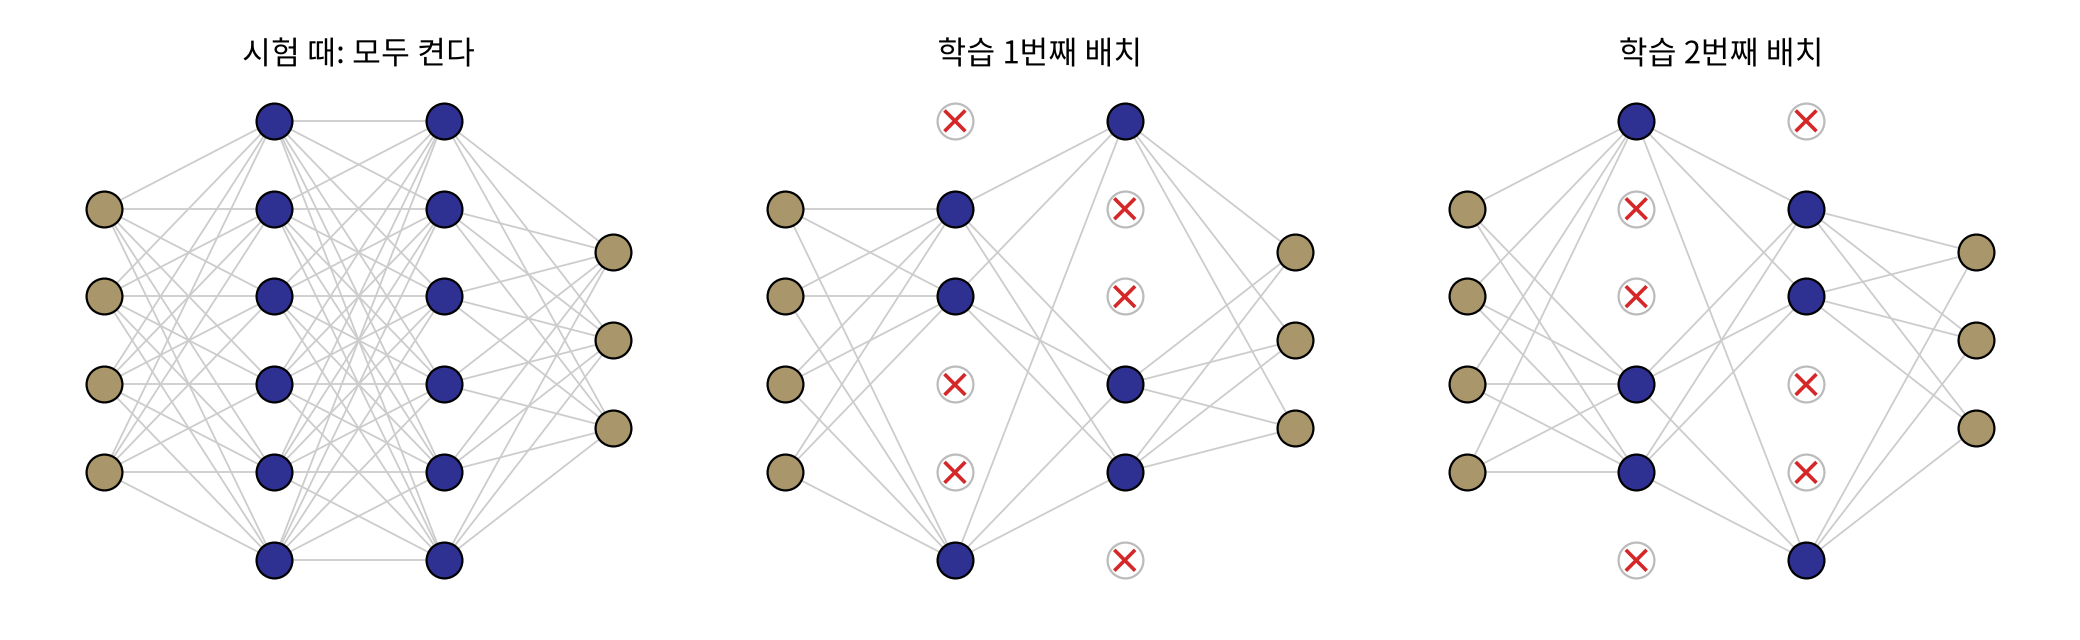
\includegraphics[width=0.92\linewidth]{do_net.png}\par\vskip0.2em
{\large 배치마다 은닉 뉴런을 확률 $p$ 로 끈다 (보통 0.5) \quad 끌 뉴런은 매번 \kb{새로}}
\vfill
\note{드롭아웃은 간단합니다. 학습할 때 배치 하나를 볼 때마다 은닉 뉴런을 확률 p로 무작위로 끕니다. 보통 p는 0.5, 절반입니다. 꺼진 뉴런은 그 배치에서는 없는 것처럼 출력이 0이고 가중치도 고쳐지지 않습니다. 중요한 건 다음 배치에서는 끌 뉴런을 새로 고른다는 겁니다. 가운데 그림과 오른쪽 그림처럼 매번 다른 뉴런이 꺼집니다. 시험할 때는 왼쪽처럼 모두 켭니다.}
\end{frame}

\section{왜}
% --- 짝꿍
\begin{frame}{왜 좋아질까 1: 짝꿍에게 기댈 수 없다}
\vfill
\centering
{\large 모두 켜져 있으면: A 의 실수를 B 가 늘 고쳐 준다 $\to$ \textbf{짝으로만} 쓸모 있는 특징}\\[0.8em]
{\large 드롭아웃: B 가 언제 꺼질지 모른다 \quad $\to$ A 는 \kb{혼자서도} 쓸모 있는 특징을 배워야 한다}\\[1.0em]
{\large 비유: 조원 절반이 매번 무작위로 빠지는 조별 과제 $\to$ 모두가 전체를 이해해야}\\[0.4em]
{\small 논문의 표현: co-adaptation (함께 맞춰지기) 을 막는다}
\vfill
\note{왜 좋아질까요? 첫 번째 설명은 짝꿍입니다. 모두 켜져 있으면 뉴런들이 서로에게 기대어 학습합니다. 뉴런 A가 엉뚱한 걸 해도 뉴런 B가 늘 고쳐 주면, 둘은 짝으로만 의미 있는 이상한 특징을 배웁니다. 학습 데이터를 외우는 데 딱 좋은 방식입니다. 드롭아웃을 쓰면 B가 언제 꺼질지 모르니, A는 혼자서도 쓸모 있는 특징을 배워야 합니다. 조별 과제에서 매번 조원 절반이 무작위로 빠진다면 모두가 과제 전체를 이해해야 하는 것과 같습니다. 논문은 이를 함께 맞춰지기, co-adaptation을 막는다고 표현했습니다.}
\end{frame}

% --- 앙상블
\begin{frame}{왜 좋아질까 2: 작은 신경망 수천 개의 앙상블}
\vfill
\centering
{\large 은닉 뉴런 12개를 켜고 끄는 조합 \quad $2^{12} = \kb{4{,}096}$ 가지}\\[0.8em]
{\large 배치마다 그중 하나를 학습한다 \quad 가중치는 모두가 \textbf{나눠 쓴다}}\\[0.8em]
{\large 시험 때 모두 켜는 것 $\approx$ 그 많은 작은 신경망의 \textbf{평균}}\\[0.8em]
{\small 랜덤 포레스트 (4주차) 가 서로 다른 나무 여럿을 평균 냈던 것과 같은 생각, 훨씬 싸게}
\vfill
\note{두 번째 설명은 앙상블입니다. 은닉 뉴런이 12개만 있어도 켜고 끄는 조합은 2의 12제곱, 4096가지입니다. 드롭아웃은 배치마다 이 중 하나의 작은 신경망을 학습하는 셈입니다. 이 작은 신경망들은 가중치를 따로 갖지 않고 모두 나눠 씁니다. 시험할 때 모두 켜는 것은 이 수많은 작은 신경망의 예측을 평균 내는 것과 비슷합니다. 4주차 랜덤 포레스트가 서로 다른 나무 여럿을 평균 냈던 것과 같은 생각인데, 신경망 수천 개를 따로 학습할 필요가 없으니 훨씬 쌉니다.}
\end{frame}

\section{쓸 때}
% --- 시험 때
\begin{frame}{시험 때는 모두 켜고, 크기를 맞춘다}
\markpage{scale}
\vfill
\centering
{\large 학습 때 절반만 켜져 있었다면 다음 층은 \textbf{절반 크기} 신호에 익숙하다}\vskip0.5em
\renewcommand{\arraystretch}{1.3}
{\Large\begin{tabular}{lcc}
 & 뉴런 출력 & 다음 층으로\\\hline
원래 & (2, 4, 6, 8) & \\
학습 ($p = 0.5$, 마스크 1, 0, 1, 0) & (2, 0, 6, 0) & \kb{$\times 2$} $\to$ (4, 0, 12, 0)\\
시험 (모두 켬) & (2, 4, 6, 8) & 그대로
\end{tabular}}\vskip0.5em
{\large 살아남은 뉴런을 $\frac{1}{1-p}$ 배 $\to$ 평균 크기가 시험 때와 같다 (inverted dropout)}
\vfill
\note{시험 때는 모든 뉴런을 켭니다. 그런데 문제가 하나 있습니다. 학습 때는 절반만 켜져 있었으니 다음 층은 평소의 절반 크기 신호에 익숙합니다. 시험 때 갑자기 모두 켜면 신호가 두 배가 됩니다. 그래서 크기를 맞춥니다. 요즘 방식은 학습 때 살아남은 뉴런의 출력을 1 나누기 1 빼기 p배, p가 0.5면 2배로 키웁니다. 출력이 2, 4, 6, 8인데 마스크가 1, 0, 1, 0이면 2, 0, 6, 0이 되고, 2배 해서 4, 0, 12, 0을 보냅니다. 평균적으로 원래와 같은 크기입니다. 시험 때는 그대로 보내면 됩니다.}
\end{frame}

% --- 실험
\begin{frame}{우리 실험: 2,000장, 100 에폭}
\vfill
\centering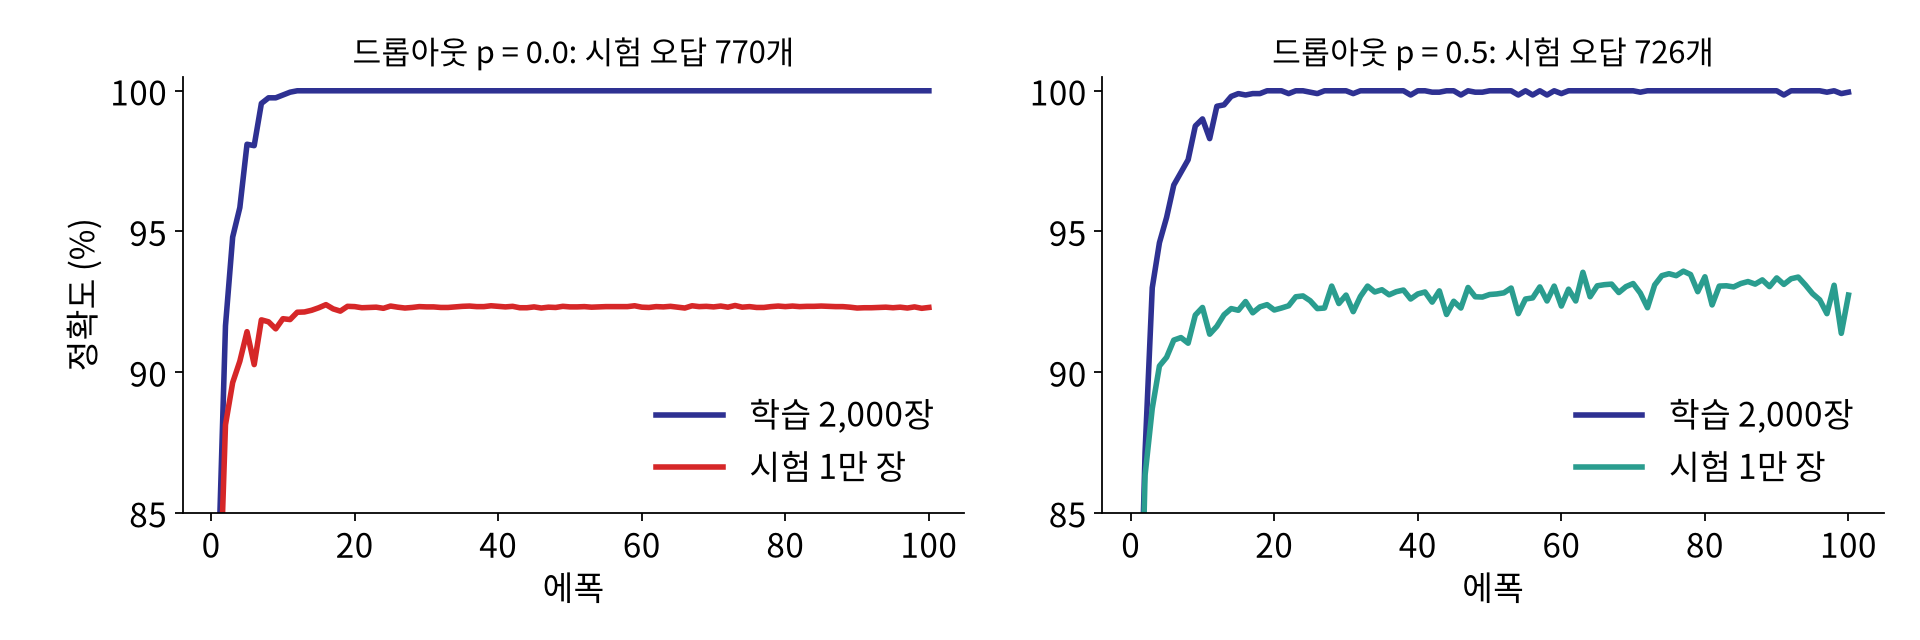
\includegraphics[width=0.86\linewidth]{do_curves.png}\par\vskip0.2em
{\large 두 신경망 모두 학습 데이터는 거의 100\% \quad 시험 오답 \kq{770} $\to$ \kb{726}}
\vfill
\note{우리 실험입니다. 드롭아웃 없이 학습하면 왼쪽처럼 학습 정확도는 100퍼센트, 시험 오답은 770개입니다. p 0.5로 드롭아웃을 쓰면 학습 정확도는 거의 같은데 시험 오답이 726개로 줄었습니다. 학습 데이터만 놓고 보면 차이가 없지만, 처음 보는 데이터에서 더 잘합니다. 외우기보다 일반적인 특징을 더 배웠다는 뜻입니다.}
\end{frame}

% --- p
\begin{frame}{얼마나 끌까: $p$}
\vfill
\centering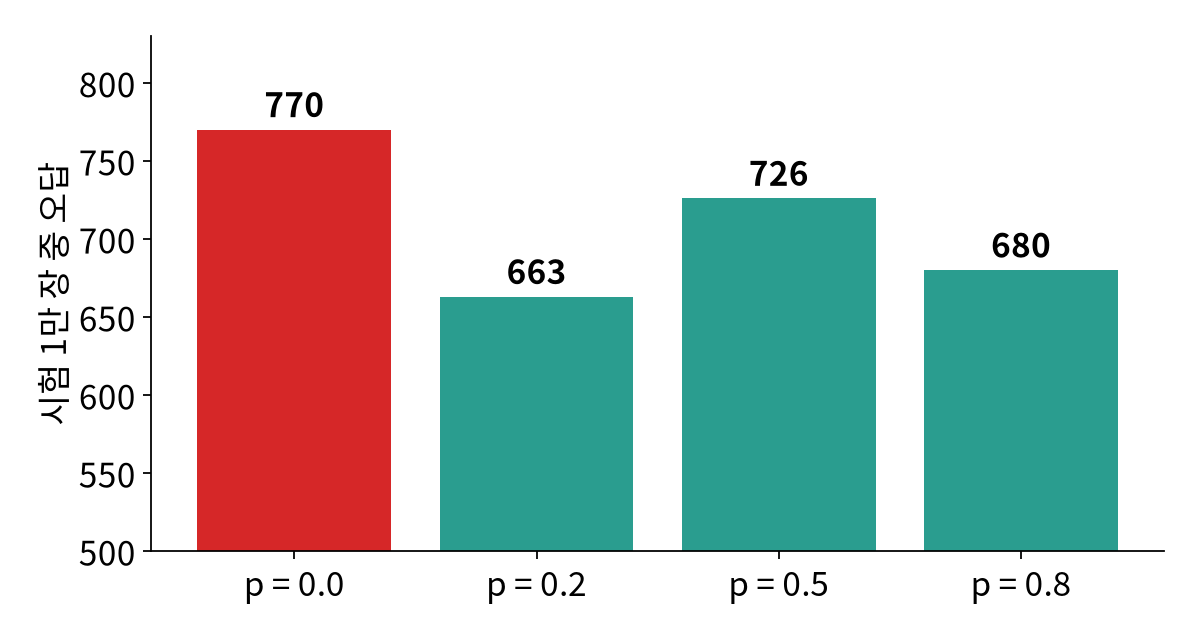
\includegraphics[width=0.52\linewidth]{do_p.png}\par\vskip0.2em
{\large $p = 0$: 770 \quad 0.2: \kb{663} \quad 0.5: 726 \quad 0.8: 680 \quad 모두 안 끈 것보다 낫다}\\[0.2em]
{\small 이 정도 차이는 시드에 따라 흔들린다 $\to$ $p$ 도 검증으로 고른다 \quad 관례: 은닉층 0.5, 입력층 0.2}
\vfill
\note{p를 바꿔 봤습니다. 0이면 770개, 0.2면 663개, 0.5면 726개, 0.8이면 680개를 틀립니다. 셋 다 드롭아웃이 없을 때보다 낫습니다. 0.2와 0.5, 0.8 사이의 차이는 시드에 따라 순서가 바뀔 정도라서 크게 믿을 만하지 않습니다. 그래서 p도 다른 손잡이처럼 검증 데이터로 고릅니다. 논문의 관례는 은닉층 0.5, 입력층 0.2입니다. 너무 크게 하면 남는 뉴런이 적어 학습이 느려지고 과소적합될 수 있습니다.}
\end{frame}

% --- 주의
\begin{frame}{쓸 때 주의: 학습 모드와 시험 모드}
\vfill
\centering
{\large PyTorch \quad \texttt{nn.Dropout(p=0.5)}}\vskip0.6em
\renewcommand{\arraystretch}{1.5}
{\large\begin{tabular}{ll}
\texttt{model.train()} & 드롭아웃 켜짐: 무작위로 끄고 $\frac{1}{1-p}$ 배\\
\texttt{model.eval()} & 드롭아웃 꺼짐: 모두 켜고 그대로
\end{tabular}}\vskip0.8em
{\large \texttt{eval()} 을 깜빡하면 \kq{예측이 매번 달라지고} 정확도가 떨어진다}\\[0.4em]
{\small 드롭아웃은 AlexNet (2012) 이 과대적합을 막는 데 썼고, 트랜스포머 (GPT · BERT) 안에도 들어 있다}
\vfill
\note{PyTorch에서는 nn.Dropout 층을 넣으면 됩니다. 주의할 점이 하나 있습니다. model.train을 부르면 드롭아웃이 켜져서 무작위로 끄고 키우고, model.eval을 부르면 꺼져서 그대로 통과시킵니다. 시험 전에 eval을 깜빡하면 예측할 때도 뉴런이 무작위로 꺼져서, 같은 그림을 넣어도 매번 답이 달라지고 정확도가 떨어집니다. 아주 흔한 실수입니다. 드롭아웃은 같은 해 AlexNet이 과대적합을 막는 데 썼고, 지금도 GPT나 BERT 같은 트랜스포머 안에 들어 있습니다.}
\end{frame}

\section{연습}
% --- 문제풀이
\begin{frame}{문제풀이}
\vfill
\begin{enumerate}
\item 은닉 뉴런 20개에 드롭아웃을 쓴다. 켜고 끄는 조합은 몇 가지인가?\vskip0.8em
\item $p = 0.25$ 일 때, 출력 (4, 8, 12, 16) 에 마스크 (1, 1, 0, 1) 이 걸렸다. 다음 층으로 보내는 값은? (inverted dropout)\vskip0.8em
\item 드롭아웃을 넣었더니 학습 정확도는 떨어지고 시험 정확도는 올랐다. 잘못된 것인가?\vskip0.8em
\item 같은 시험 그림을 두 번 넣었더니 답이 달랐다. 무엇을 빼먹었을까?
\end{enumerate}
\vfill
\note{1번 답. 2의 20제곱, 약 104만 가지입니다. 2번 답. 살아남은 값을 1 나누기 0.75, 약 1.33배 하니 5.33, 10.67, 0, 21.33입니다. 3번 답. 정상입니다. 학습 데이터를 덜 외우고 일반화가 좋아진 겁니다. 학습 때는 뉴런이 꺼져 있어서 학습 정확도가 낮게 보이기도 합니다. 4번 답. model.eval입니다.}
\end{frame}

% --- 실습
\begin{frame}{실습}
\vfill
\centering\begin{tabular}{rl}
\large 1 & 드롭아웃 직접 구현 (마스크 + $\frac{1}{1-p}$) $\to$ 평균 크기가 유지되는지 확인\\[0.5em]
\large 2 & MNIST 2,000장: 드롭아웃 없음 vs $p = 0.5$ 학습 곡선\\[0.5em]
\large 3 & \texttt{eval()} 을 깜빡하면? 같은 그림 예측이 매번 달라지는 것 확인
\end{tabular}\vskip1em
MNIST (LeCun, Cortes, Burges; torchvision) \\[0.4em]\href{https://colab.research.google.com/github/SuminHan/book-ml/blob/main/slides/v2/ml1/week09/dropout/lab/dropout.ipynb}{\textcolor{ksagolddk}{▶ Colab에서 실습 노트북 열기}}
\vfill
\note{실습은 세 부분입니다. 첫째, 마스크와 크기 보정으로 드롭아웃을 직접 구현하고, 평균 크기가 유지되는지 확인합니다. 둘째, MNIST 2000장으로 드롭아웃이 없을 때와 p 0.5일 때 학습 곡선을 비교합니다. 셋째, eval을 깜빡하면 같은 그림의 예측이 매번 달라지는 것을 직접 봅니다.}
\end{frame}

\section{정리}
% --- 정리
\begin{frame}{정리}
\vfill
\centering\large\begin{tabular}{l}
\textbf{Dropout} \quad 학습 때 배치마다 뉴런을 확률 $p$ 로 무작위로 끈다 (Hinton 외, 2012)\\[0.5em]
짝꿍에게 기대지 않는 특징 \quad 작은 신경망 수천 개의 앙상블\\[0.5em]
시험 때는 모두 켠다 \quad 학습 때 살아남은 뉴런을 $\frac{1}{1-p}$ 배\\[0.5em]
MNIST 2,000장: 오답 770 $\to$ 663 $\sim$ 726 \quad \texttt{train()} / \texttt{eval()} 꼭 구분
\end{tabular}
\vfill
\note{정리합니다. 드롭아웃은 학습 때 배치마다 뉴런을 확률 p로 무작위로 끄는 방법입니다. 뉴런이 짝꿍에게 기대지 않고 혼자서도 쓸모 있는 특징을 배우게 되고, 작은 신경망 수천 개를 평균 내는 앙상블 효과도 있습니다. 시험 때는 모두 켜고, 크기를 맞추기 위해 학습 때 살아남은 뉴런을 1 나누기 1 빼기 p배 합니다. 우리 실험에서는 오답이 770개에서 663에서 726개로 줄었습니다. 그리고 train과 eval을 꼭 구분해서 씁니다.}
\end{frame}
\end{document}
